% -*- compile-command: "latexmk -pdf notes.tex" -*-
\documentclass{article}

\input{template}

\author{Sam Price}
\date{}
\title{Graph Theory}

\begin{document}

\section{What is a graph?}
A graph $G$ is a collection of both \emph{vertices} and \emph{edges}, denoted $G[V]$ and $G[E]$ respectively.
When the relevant graph is obvious, they may be referred as simply $V$ and $E$.
The vertices are normally numbered, but may be represented by any mathematical object. Edges on the other hand,
are always pairs of vertices such as $(v_{1}, v_{2})$ where $v_{1},v_{2} \in G[V]$.

There are three main types of edges, namely bidirectional, unidirectional (these are called \emph{directed graphs}, or \emph{digraphs})
or one of those previous types with an associated number. The latter is referred to as \emph{weighted graphs}, which is more common in computer science.

\section{Classification of Graphs}
There are many different and complex classifications of graphs. Note that the subscript $n$ is usually equal to the number of relevant vertices, or
if the whole graph is involved then $n = \abs{V}$.
\begin{itemize}
  \item Path ($P_{n}$)

        A \emph{path} is a graph (or subgraph, but that's for later!) which looks like a single line of connected vertices,
        where all but two vertices are connected to two others, and the last two only connected to one each.

        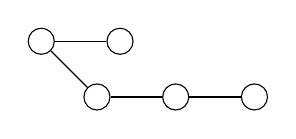
\begin{tikzpicture}[main/.style = {draw, circle}]
          \node[main] (1) {};
          \node[main] (2) [left of = 1] {};
          \node[main] (3) [below right of = 2]{};
          \node[main] (4) [right of = 3]{};
          \node[main] (5) [right of = 4]{};
          \draw (1) -- (2);
          \draw (2) -- (3);
          \draw (3) -- (4);
          \draw (4) -- (5);
        \end{tikzpicture}

  \item Cycle ($C_{n}$)

        A cycle is a ``loop'', or a path which connects back to itself.

        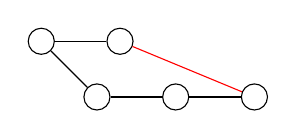
\begin{tikzpicture}[main/.style = {draw, circle}]
          \node[main] (1) {};
          \node[main] (2) [left of = 1] {};
          \node[main] (3) [below right of = 2]{};
          \node[main] (4) [right of = 3]{};
          \node[main] (5) [right of = 4]{};
          \draw (1) -- (2);
          \draw (2) -- (3);
          \draw (3) -- (4);
          \draw (4) -- (5);
          \draw[color=red] (5) -- (1);
        \end{tikzpicture}

  \item Complete ($K_{n}$)

        This is simply the graph with $n$ vertices where every vertex is connected to all the others. $K$ chosen, since $C$ was taken by the cycles.

        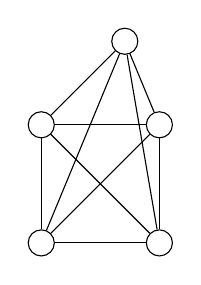
\begin{tikzpicture}[node distance = 15mm, main/.style = {draw, circle}]
          \node[main] (1) {};
          \node[main] (2) [below left of = 1] {};
          \node[main] (3) [below of = 2]{};
          \node[main] (4) [right of = 3]{};
          \node[main] (5) [above of = 4]{};
          \draw (1) -- (2);
          \draw (1) -- (3);
          \draw (1) -- (4);
          \draw (1) -- (5);
          \draw (2) -- (3);
          \draw (2) -- (4);
          \draw (2) -- (5);
          \draw (3) -- (4);
          \draw (3) -- (5);
          \draw (4) -- (5);
        \end{tikzpicture}
\end{itemize}

\end{document}
